% begin module velocity-ex3
\begin{frame}
\frametitle{Velocities}
\begin{example}[Example 3, p. 137]
Suppose a ball is dropped from the upper deck of the CN Tower, 450m above the ground.  What is the velocity of the ball after 5 seconds?
\end{example}
\begin{itemize}
\item<2->  We need to know what ``instantaneous'' velocity is.
\item<3->  Let $f(x)$ denote the displacement of an object at time $x$.
%\item<4->  The slope of the secant from $(a, f(a))$ to $(x, f(x))$ is the average velocity over the interval $[a, x]$.
%\item<5->  The slope of the tangent line at $a$ is the instantaneous velocity at the time $a$.
\end{itemize}
\begin{center}
\begin{columns}[c]
\column{.4\textwidth}
\ \uncover<4->{%
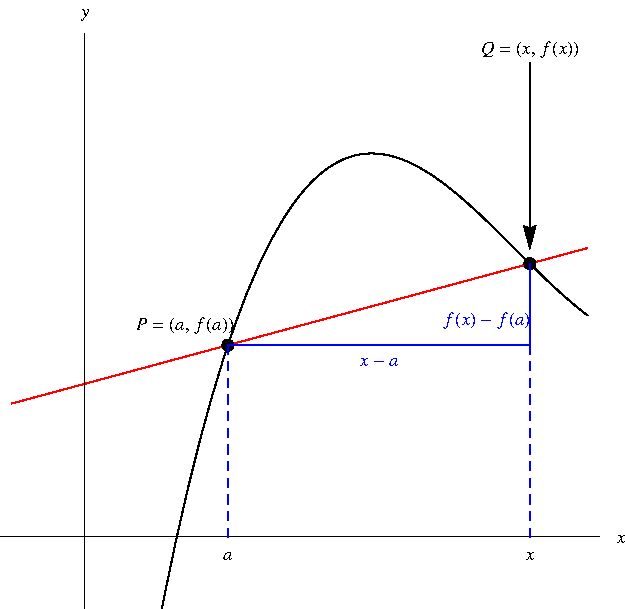
\includegraphics[height=3.5cm]{derivatives/pictures/03-01-secanta.pdf}%

Slope of secant\\ $ = $ average velocity
}%
\column{.4\textwidth}
\ \uncover<5->{%
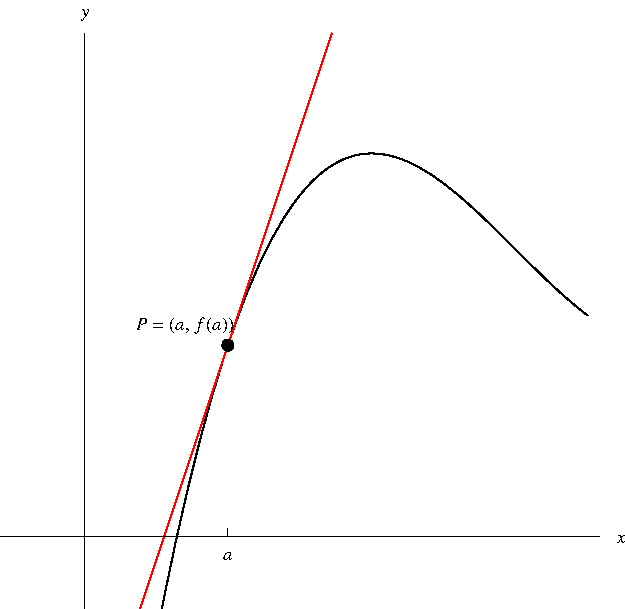
\includegraphics[height=3.5cm]{derivatives/pictures/03-01-tangent.pdf}%

Slope of tangent\\ $ = $ instantaneous velocity
}%
\end{columns}
\end{center}
\end{frame}

\begin{frame}
\begin{example}[Example 3, p. 137]
Suppose a ball is dropped from the upper deck of the CN Tower, 450m above the ground.  What is the velocity of the ball after 5 seconds?
\begin{itemize}
\item<2->  The distance $f(x)$ (in meters) that the ball has fallen at time $x$ (in seconds) follows Galileo's law: $f(x) = 4.9x^2$.
\item<3->  Let $v(a)$ be its velocity at time $a$.
\end{itemize}
\abovedisplayskip=0pt
\belowdisplayskip=0pt
\begin{align*}
\uncover<4->{%
v(a)
}%
& \uncover<4->{ = } %
\uncover<4->{%
\lim_{h\rightarrow 0}\frac{f(a+h)-f(a)}{h}
}  \uncover<5->{ = } \uncover<5->{%
\lim_{h\rightarrow 0}\frac{4.9(a+h)^2-4.9a^2}{h}
}\\%
& \uncover<6->{ = } %
\uncover<6->{%
\lim_{h\rightarrow 0}\frac{4.9(a^2+2ah+h^2)-4.9a^2}{h}
}\\%
& \uncover<7->{ = } %
\uncover<7->{%
\lim_{h\rightarrow 0}\frac{4.9(2ah+h^2)}{h}
}\\%
& \uncover<8->{ = } %
\uncover<8->{%
\lim_{h\rightarrow 0}4.9(2a+h)
}%
\uncover<9->{%
 = 9.8a
}%
\end{align*}
\uncover<10->{%
Therefore the velocity after 5s is $v(5) = 9.8(5) = 49$m/s.
}%
\end{example}
\end{frame}
% end module velocity-ex3
